\clearpage
\section{Funktionsweise}\label{sec:Funktionsweise}
Folglich soll die Funktionsweise einer differenziellen Kryptoanalyse auf eine Runde vom Data Encryption Standard (DES) erläutert werden. Es wird nur die rechte Seite einer DES-Runde betrachtet, womit die Klartexte 32 Bit lang sind. 
Wie der Name es schon andeutet, wird bei diesem Verfahren die Differenz aus zwei Klartexten, in diesem Beispiel mit $P_{1}$ und $P_{2}$ bezeichnet, verwendet. Die Differenz wird üblicherweise mit $P'$ bezeichnet und folgt aus einer XOR-Verknüpfung der Klartexte, also $P' = P_{1} \oplus P_{2}$.
Funktionen wie Expansionen, Permutationen oder XOR-Verknüpfen haben keine Einfluss auf die Differenz der Texte. Die Differenz kann also fast durch die gesamte Feistelstruktur beobachtet werden. Die Abbildung \ref{fig:DES_Differenz} zeigt wie sich eine Differenz durch das Netzwerk verhält. 
Die Ausgangspermutation und die XOR-Verknüpfung mit der linken Seite ($L_{0}$) wurden nicht in der Abbildung dargestellt da sie bei einer Runde von DES nicht von Bedeutung sind.

\begin{figure}[h]
	\centering
	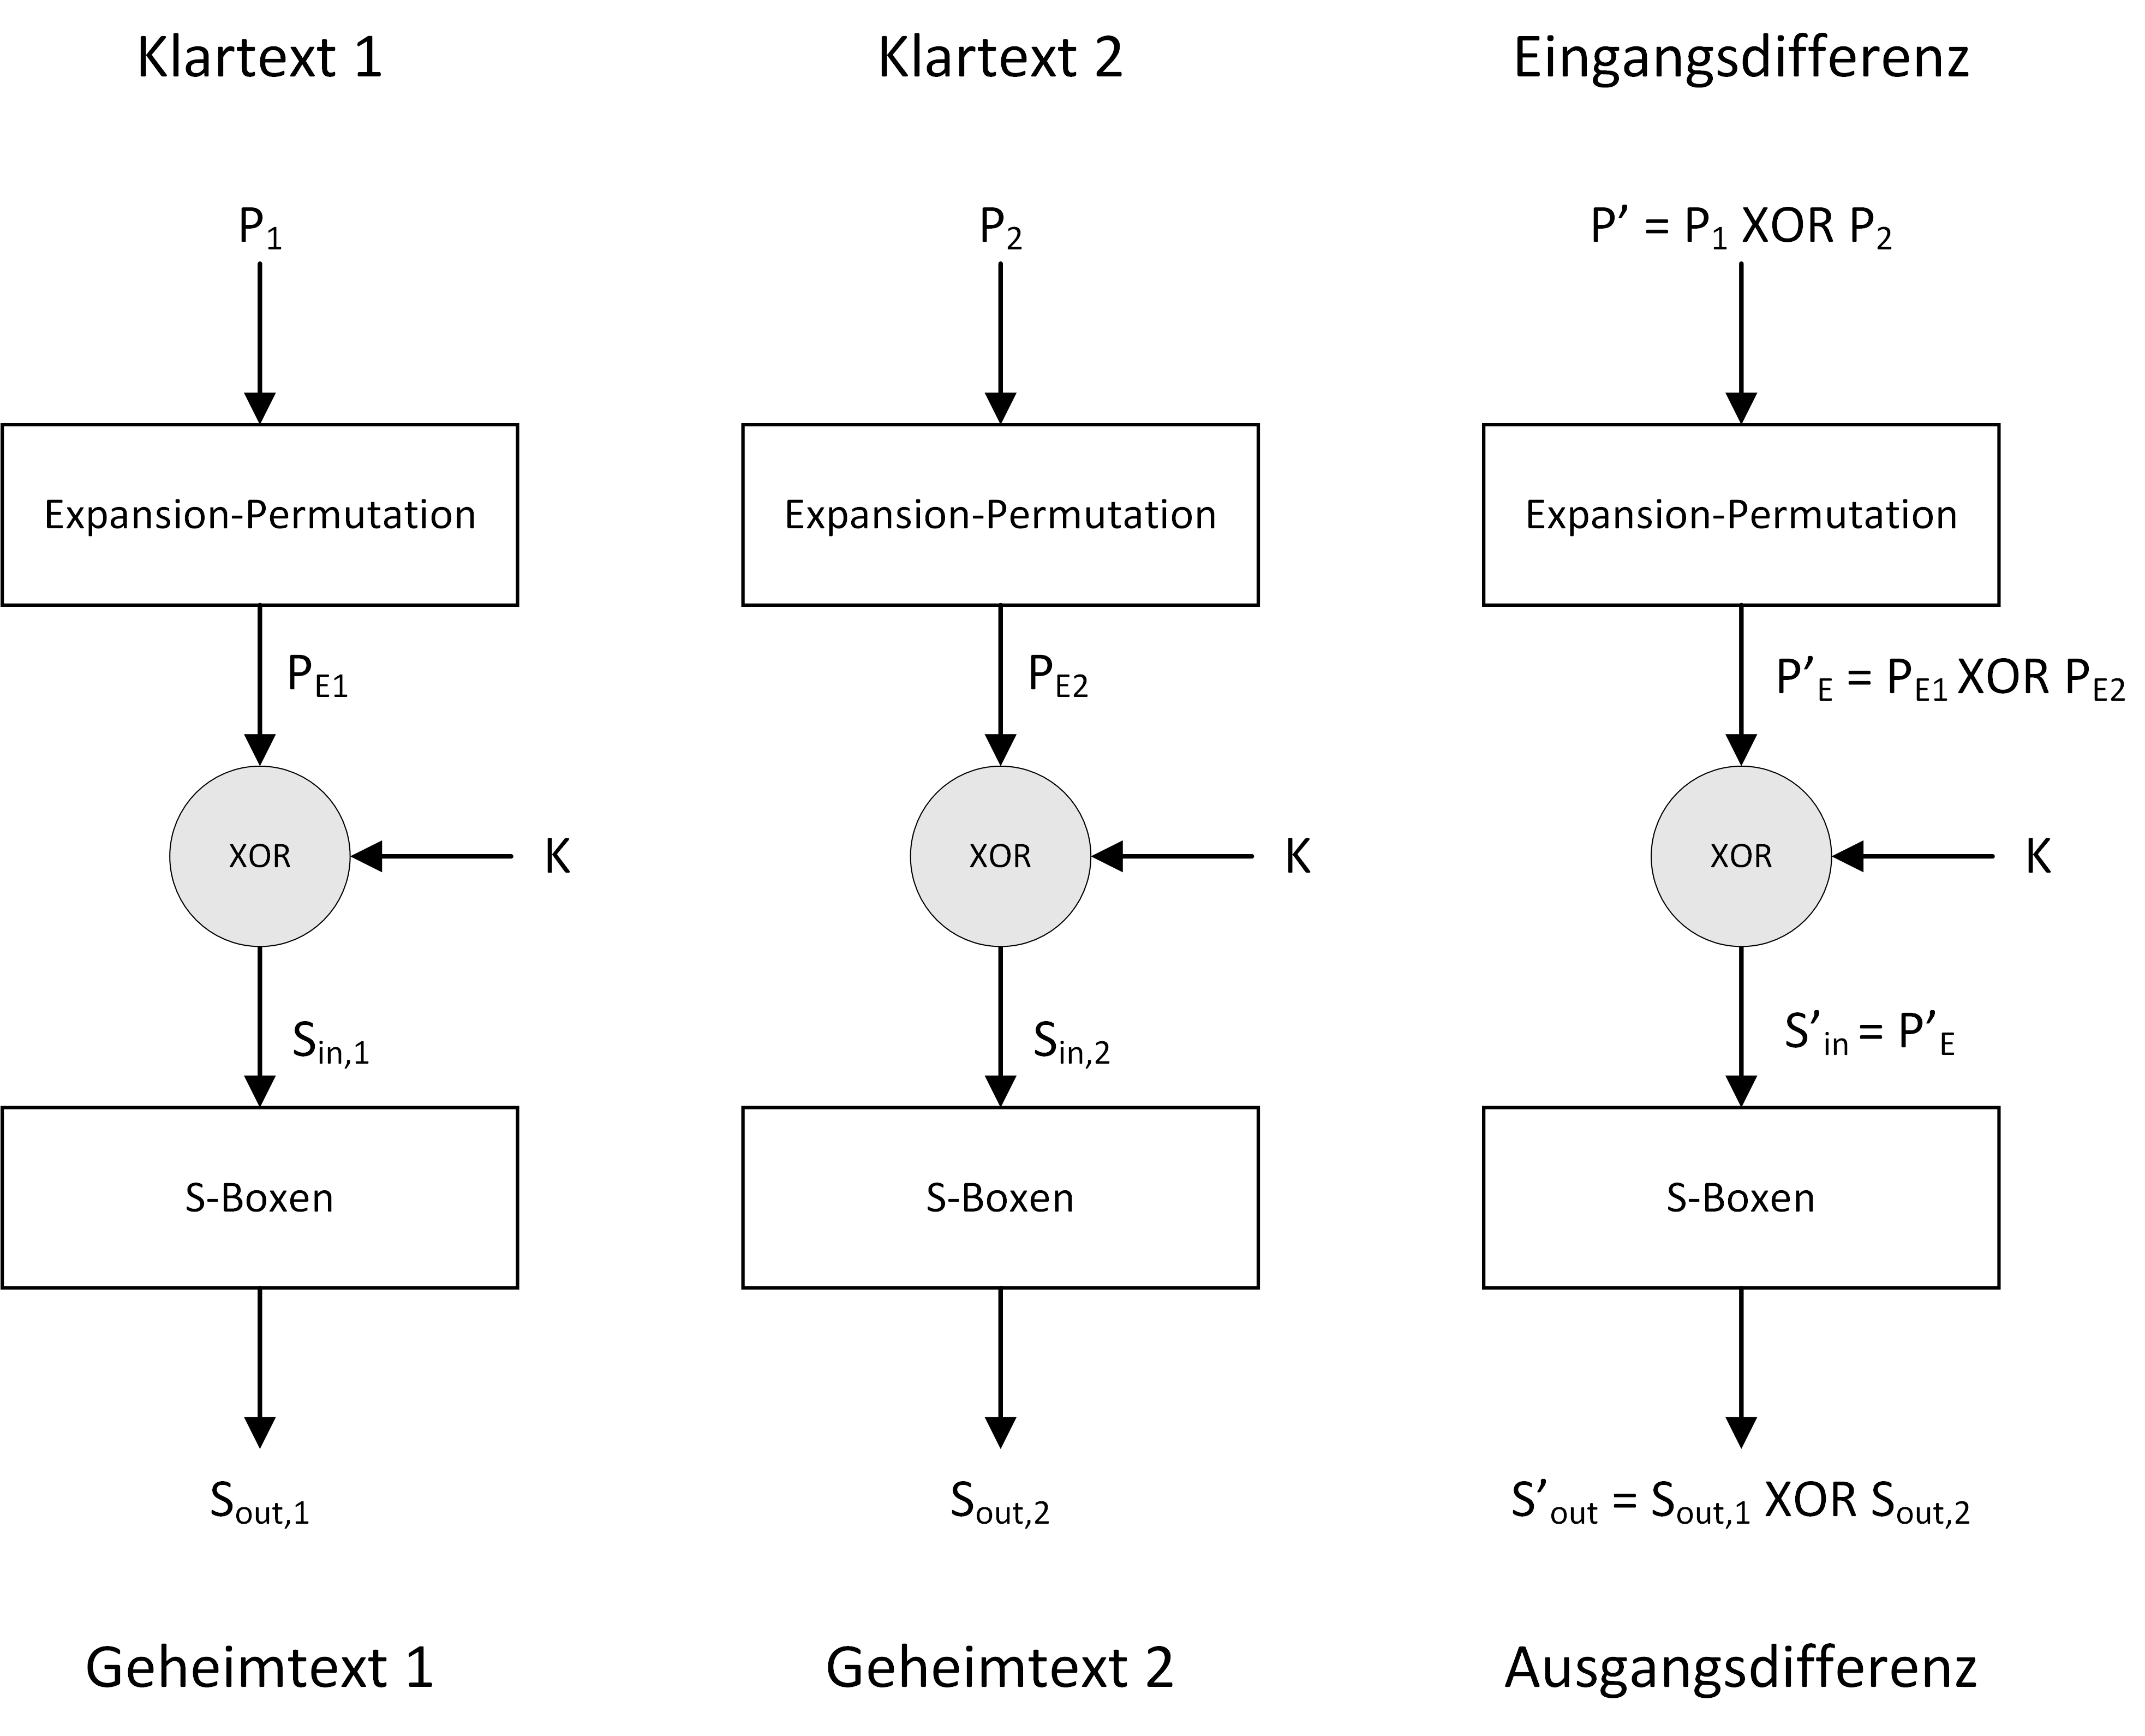
\includegraphics[width=1.0\linewidth]{graphics/DES_Differenz.jpg}
	\caption{Verhalten von Klartext 1, 2 und der Differenz davon durch die Feistelstruktur einer Runde von DES \cite{the_morpheus_tutoials_kryptographie_2016}}
	\label{fig:DES_Differenz}
\end{figure}

Die Eingangswerte $S_{in,1}$ und $S_{in,2}$ der S-Boxen sind ohne Schlüssel nicht bekannt. Bei der Spalte \glqq Differenz\grqq{} ist dieser Eingang $S'_{in}$ aber bekannt. Eine doppelte XOR-Verknüpfung mit dem Schlüssel hebt sich auf. Mit anderen Worten ist: 

\begin{equation}\label{equ:Schluessel_Differenz}
S'_{in} = S_{in,1} \oplus S_{in,2} = (P_{E,1} \oplus K) \oplus (P_{E,2} \oplus K) = P_{E,1} \oplus P_{E,2} = P'_{E} 
\end{equation}


Mit dieser Eigenschaft können die S-Boxen genauer analysiert werden. 
Wie bereits in der Einleitung erwähnt, sind die acht S-Boxen nicht-lineraren Funktion. Um diese zu umgehen kann mit Wahrscheinlichkeiten gearbeitet werden.
Anhand der öffentlich zugänglichen S-Boxen kann eine Differenzenverteilungstabelle aufgestellt werden. In dieser wird für jede Eingangsdifferenz die Zahl Wertepaar gegeben welche eine bestimmte Ausgangsdifferenz erzeugen. 
Es gibt bei DES $2^{6} = 64$ verschieden mögliche Eingangsdifferenzen pro S-Box. Jede Eingangsdifferenz kann mit 64 verschiedenen Wertepaare erzeugt werden. Als Beispiel: für eine Eingangsdifferenz von $34_{h}$ (Hexadezimalzahl) gibt es laut Differenzenverteilungstabelle nur zwei von den 64 Wertepaar die, beim Durchqueren der S-Boxen 1, eine Ausgangsdifferenz von $04_{h}$ erzeugen \cite{noauthor_differenzielle_2019}\cite{biham_differential_1990}. 

Da bei einer chosen plaintext attack die Ausgangsdifferenz bekannt ist, können die möglichen Eingangswertepaare $(S_{in,1}, S_{in,2})$ in einer weiteren Tabelle abgelesen werden. Entsprechend der Differenzenverteilungstabelle gibt es mehr oder weniger solche möglichen Eingangspaar.
Für das Beispiel mit der Eingangsdifferenz $34_{h}$ und der Ausgangsdifferenz $04_{h}$ gibt es die 2 Wertepaare $(S_{in,1}, S_{in,2}) = (13_{h}, 27_{h})$ oder $(S_{in,1},S_{in,2}) = (27_{h}, 13_{h})$. Wäre die Ausgangsdifferenz $02_{h}$ bei einer Eingangsdifferenz von $34_{h}$ würde es 16 mögliche Wertepaare geben. 

Da nun die Eingangswerte bekannt sind, kann der Schlüssel wie folgt berechnet werden:
\begin{equation}\label{equ:Schluessel_Loesung}
K = P_{E,1} \oplus S_{in,1} = P_{E,2} \oplus S_{in,2}
\end{equation}

Weil nicht mit Sicherheit gesagt werden kann welches Wertepaar $(S_{in,1}, S_{in,2})$ das richtige ist, gibt es bei diesem Beispiel zwei mögliche Schlüssel. Es müssten die anderen S-Boxen betrachtet oder mehrere Durchgänge durchgeführt werden, um den falschen Schlüssel auszuschliessen. 

\subsection{Mehrere Runden von DES}\label{subsec:Mehrere_Runden}
Bis jetzt wurde lediglich eine Runde von DES betrachtet. Es braucht nur wenige Klartext-Geheimtext-Paare damit der Schlüssel für eine Runde ermittelt werden kann. Bei mehr als 2 Runden von DES können nicht mehr alle wichtigen Differenzen in der Feistelstruktur ermittelt werden. 
An dieser Stelle kommen die Runden-Charakteristik ins Spiel. Da die Zwischenresultate nicht zur Verfügung stehen, werden sich wiederholende Strukturen gesucht, sogenannte iterative Charakteristiken. Diese können sich nach eine oder mehrere Runden wiederholen. Die Abbildung \ref{fig:Charakteristik} zeigt eine Zweirunden-Charakteristik. 

\begin{figure}[h]
	\centering
	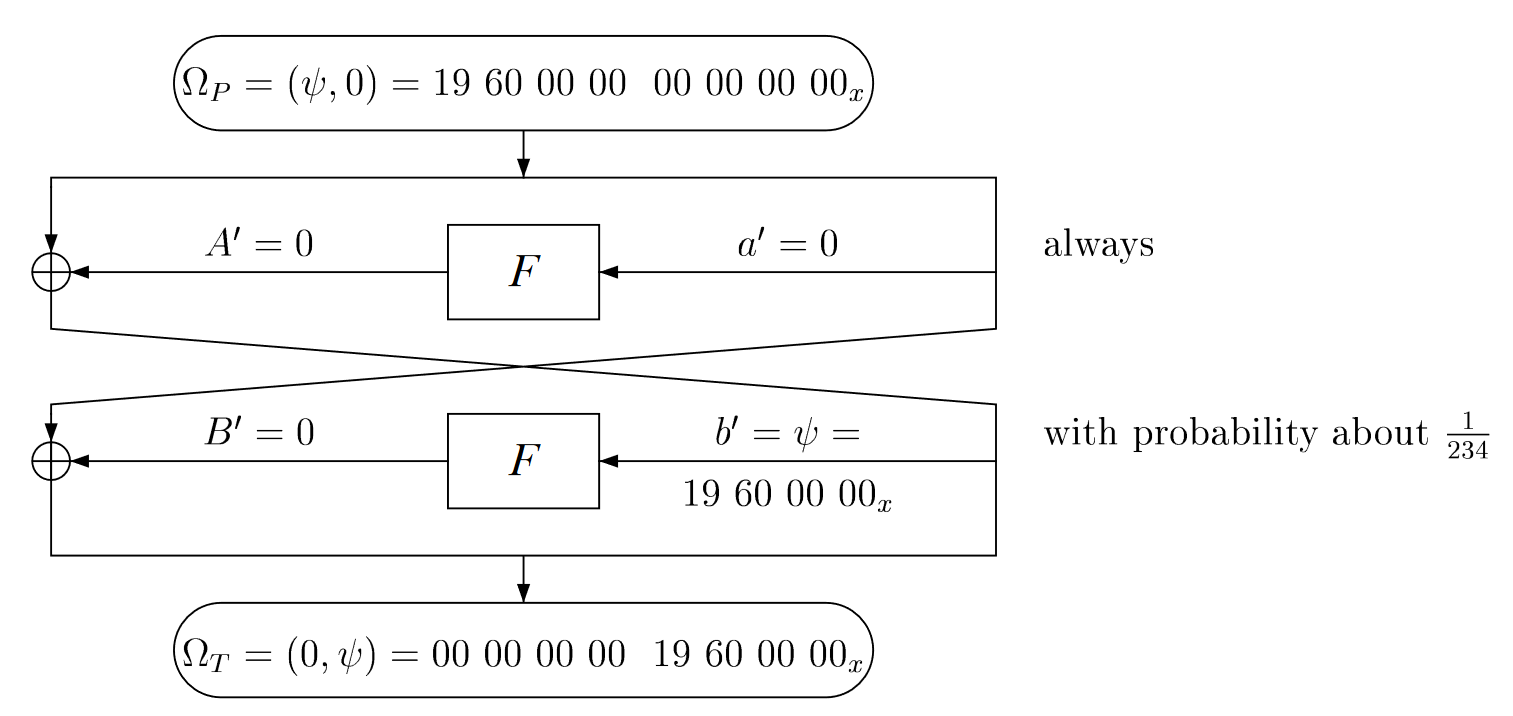
\includegraphics[width=1.0\linewidth]{graphics/Charakteristik.png}
	\caption{Dies ist eine Zweirunden-Charakteristik für die differenzielle Kryptoanalyse bei mehr als zwei Runden von DES. Die Eingangsdifferenz wiederholt sich nach zwei Runden in der Feistelstruktur \cite{biham_differential_1990}.}
	\label{fig:Charakteristik}
\end{figure}

Die Wahrscheinlichkeiten (im Bild \ref{fig:Charakteristik} auf der rechten Seite: $p_{1} = 1$ = always und $P_{2} = 1/234$) stammen aus den Differenztabellen für alle 8 S-Boxen. Anders gesagt, gibt es eine Eingangsdifferenz von 234 welche am Ausgang die selbe Differenz hat. Falls diese gefunden wird, kann in der Feistelstruktur zurück gerechnet werden und die Rundenschlüssel somit ermittelt werden. 
Es gibt andere Eingangsdifferenzen welche sich nach zwei Runden wiederholen, entsprechend nicht nur $\Omega_{P} = 19600000\ 00000000$,  jedoch sind diese eher selten. Die meisten davon sind gut bei wenig Runden von DES (bis 9 Runden).
Das Beipiel in Abbildung \ref{fig:Charakteristik} kann aber bis 15 Runden von DES gebraucht werden. 
Umso mehr Runden der Verschlüsselungsalgorithmus hat, desto unwahrscheinlicher ist es ein richtiges Paar zu finden. Die Wahrscheinlichkeiten der Charakteristiken werden miteinander Multipliziert.
Bei 16 Runden wird die Wahrscheinlichkeit das richtige Paar zu finden so klein, dass ein Brut-force Attacke genau so schneller wäre.
Die differenzielle Kryptoanalyse ist hingegen effizient bei anderen DES-ähnliche Kryptosysteme. Verschlüsselungsverfahren wie die Achtrunden-Variante von Lucifer (Verschlüsselungsverfahren entworfen durch IBM vor DES) oder FEAL-4 / FEAL-8 können zum Beispiel mit der vorgestellten Methode gebrochen werden. FEAL mit weniger als 32 Runden können teilweise gebrochen werden \cite{biham_differential_1990}.













